%%%%%%%%%%%%%%%%%%%%%%%%%%%%%%%%%%%%%%%%%%%%%%%%%%%%%%%%%%%%%%%%%%
%  = PREAMBLE =
% The preamble of a LaTeX document is the set of commands that 
%    precede the \begin{document} line.  It sets up the style of 
%    the document.
%%%%%%%%%%%%%%%%%%%%%%%%%%%%%%%%%%%%%%%%%%%%%%%%%%%%%%%%%%%%%%%%%%

\documentclass[aps,twocolumn, secnumarabic,balancelastpage,amsmath,amssymb,nofootinbib,floatfix]{revtex4-1}

\usepackage{graphicx}      % tools for importing graphics
\usepackage{tikz}
\usepackage{tikz-feynman}  % Requires TikZ-Feynman package
\usepackage{parskip}
\usepackage[colorlinks=true]{hyperref}  % this package should be added after 
                                        % all others.
                                        % usage: \url{http://web.mit.edu/8.13}

\setlength{\parskip}{5pt}
\usetikzlibrary{decorations.pathmorphing}

%%%%%%%%%%%%%%%%%%%%%%%%%%%%%%%%%%%%%%%%%%%%%%%%%%%%%%%%%%%%%%%%%%%
% And now, begin the document...
%%%%%%%%%%%%%%%%%%%%%%%%%%%%%%%%%%%%%%%%%%%%%%%%%%%%%%%%%%%%%%%%%%%

\begin{document}

\title{Random Number Generator from Atomospheric Muon Detection}% \author{Vinh Tran}
% \email{vinhtran@mit.edu}
\author{Yongao Hu}
\email{yongao@mit.edu}
\date{\today}
\affiliation{MIT Department of Physics}


\begin{abstract}
This report presents a statistical analysis on the random nature of atmospheric muon detection. The analysis is based on the data collected by the Cosmic Muon Detector at MIT, which detects atmospheric muons produced by cosmic rays interacting with the Earth's atmosphere. The data is analyzed using statistical methods to determine the random nature of the muon detection process. The results show that the muon detection process is indeed random. 
\end{abstract}

\maketitle

\section{Introduction}
Cosmic rays are high-energy particles that originate from outer space and interact with the Earth's atmosphere, producing secondary particles such as muons. These muons can be detected by ground-based detectors, such as the Cosmic Watch detectors. 

Random number generators produces numbers that are uniformly distributed over a range of values. These random numbers are used in various applications, including cryptography, simulations, and statistical analysis. We aim to test if the muon detection process can be used as a source of true random numbers. 

In theory, atomospheric muons are produced by cosmic rays interacting with the Earth's atmosphere. The muons are produced at a high altitude and travel through the atmosphere before reaching the ground. The muons are produced at a rate that is proportional to the intensity of the cosmic rays, which is random in nature. 

\section{Experimental Setup}
The Cosmic Muon Detector at MIT consists of a scintillator that emits light when a muon passes through it, and a photomultiplier tube (PMT) that detects the light and produces an electrical signal. The PMT signal is then processed to determine the time and energy of the muon detection event \cite{axani2024cosmicwatch}. We only count the event if two detectors are triggered at the same time. The coincidence events indicate that the muon passed through both detectors. 

The data is collected over a period of time, and the number of muon detection events is recorded. The data is then analyzed using statistical methods to determine the random nature of the muon detection process.

We also take data at different incident angle of the detectors to see if the angle has any effect on the random nature of the data. 

\section{Data Analysis}
In order to analyze the random nature of the data, we take the timestamp of the events and convert them to 0 if the timestamp is even and 1 if the timestamp is odd \cite{axani2024cosmicwatch}. This gives us a binary sequence of 0s and 1s. We then calculate the probability of getting a 1 in the sequence, which should be close to 0.5 if the data is random. 

In order to test the long-range correlation of the data, we calculate the autocorrelation function of the binary sequence. The autocorrelation function is defined as:
\begin{equation}
R(\tau) = \frac{1}{N} \sum_{i=0}^{N-\tau-1} (x_i - \bar{x})(x_{i+\tau} - \bar{x})
\end{equation}
where $N$ is the total number of events, $x_i$ is the binary sequence, $\bar{x}$ is the mean of the binary sequence, and $\tau$ is the time lag. The autocorrelation function should decay to zero if the data is random.

We also conduct a sequence test to check for the presence of long-range correlations in the data. We convert the consecutive events into an $n$-bit binary sequence, where $n$ is the number of bits in each number. We then plot the probability of each bit against the possible number that can be generated by the sequence. The plot should show a uniform distribution if the data is random.

Moreover, we also conduct a compression test to check for the presence of long-range correlations in the data. We compress the binary sequence using a simple compression algorithm, such as run-length encoding, and then calculate the compression ratio. The compression ratio should be close to 1 if the data is random.

We also calculate the entropy of the binary sequence using the Shannon entropy formula:
\begin{equation}
H(X) = -\sum_{i=0}^{n-1} p(x_i) \log_2 p(x_i)
\end{equation}
where $p(x_i)$ is the probability of each symbol in the sequence. The entropy should be close to 1 if the data is random.

We also conduct a Lempel-Ziv complexity test to check for the presence of long-range correlations in the data. The Lempel-Ziv complexity is a measure of the complexity of a sequence, and it is defined as the number of distinct substrings in the sequence. The Lempel-Ziv complexity should be close to 1 if the data is random.
The Lempel-Ziv complexity is calculated using the formula:
\begin{equation}
L(Z) = \sum_{i=0}^{n-1} \frac{1}{2^i} \sum_{j=0}^{n-i-1} (x_j - x_{j+i})
\end{equation}
where $n$ is the length of the sequence, $x_j$ is the $j$-th symbol in the sequence, and $i$ is the length of the substring. The Lempel-Ziv complexity should be close to 1 if the data is random. 

To model the angular depedence on the random nature of the data, we take data at different angles and repeat the same analysis. We then conduct a $\chi^2$ test to check for the correlation between the angle and probability of getting a 1 in the sequence. 



\section{Results}
Here we present the results of the analysis. Firstly, we plot the count of 1 and 0 in the binary sequence. The plot shows that the count of 1 and 0 is roughly equal, indicating that the data is random.
\begin{figure}
\centering
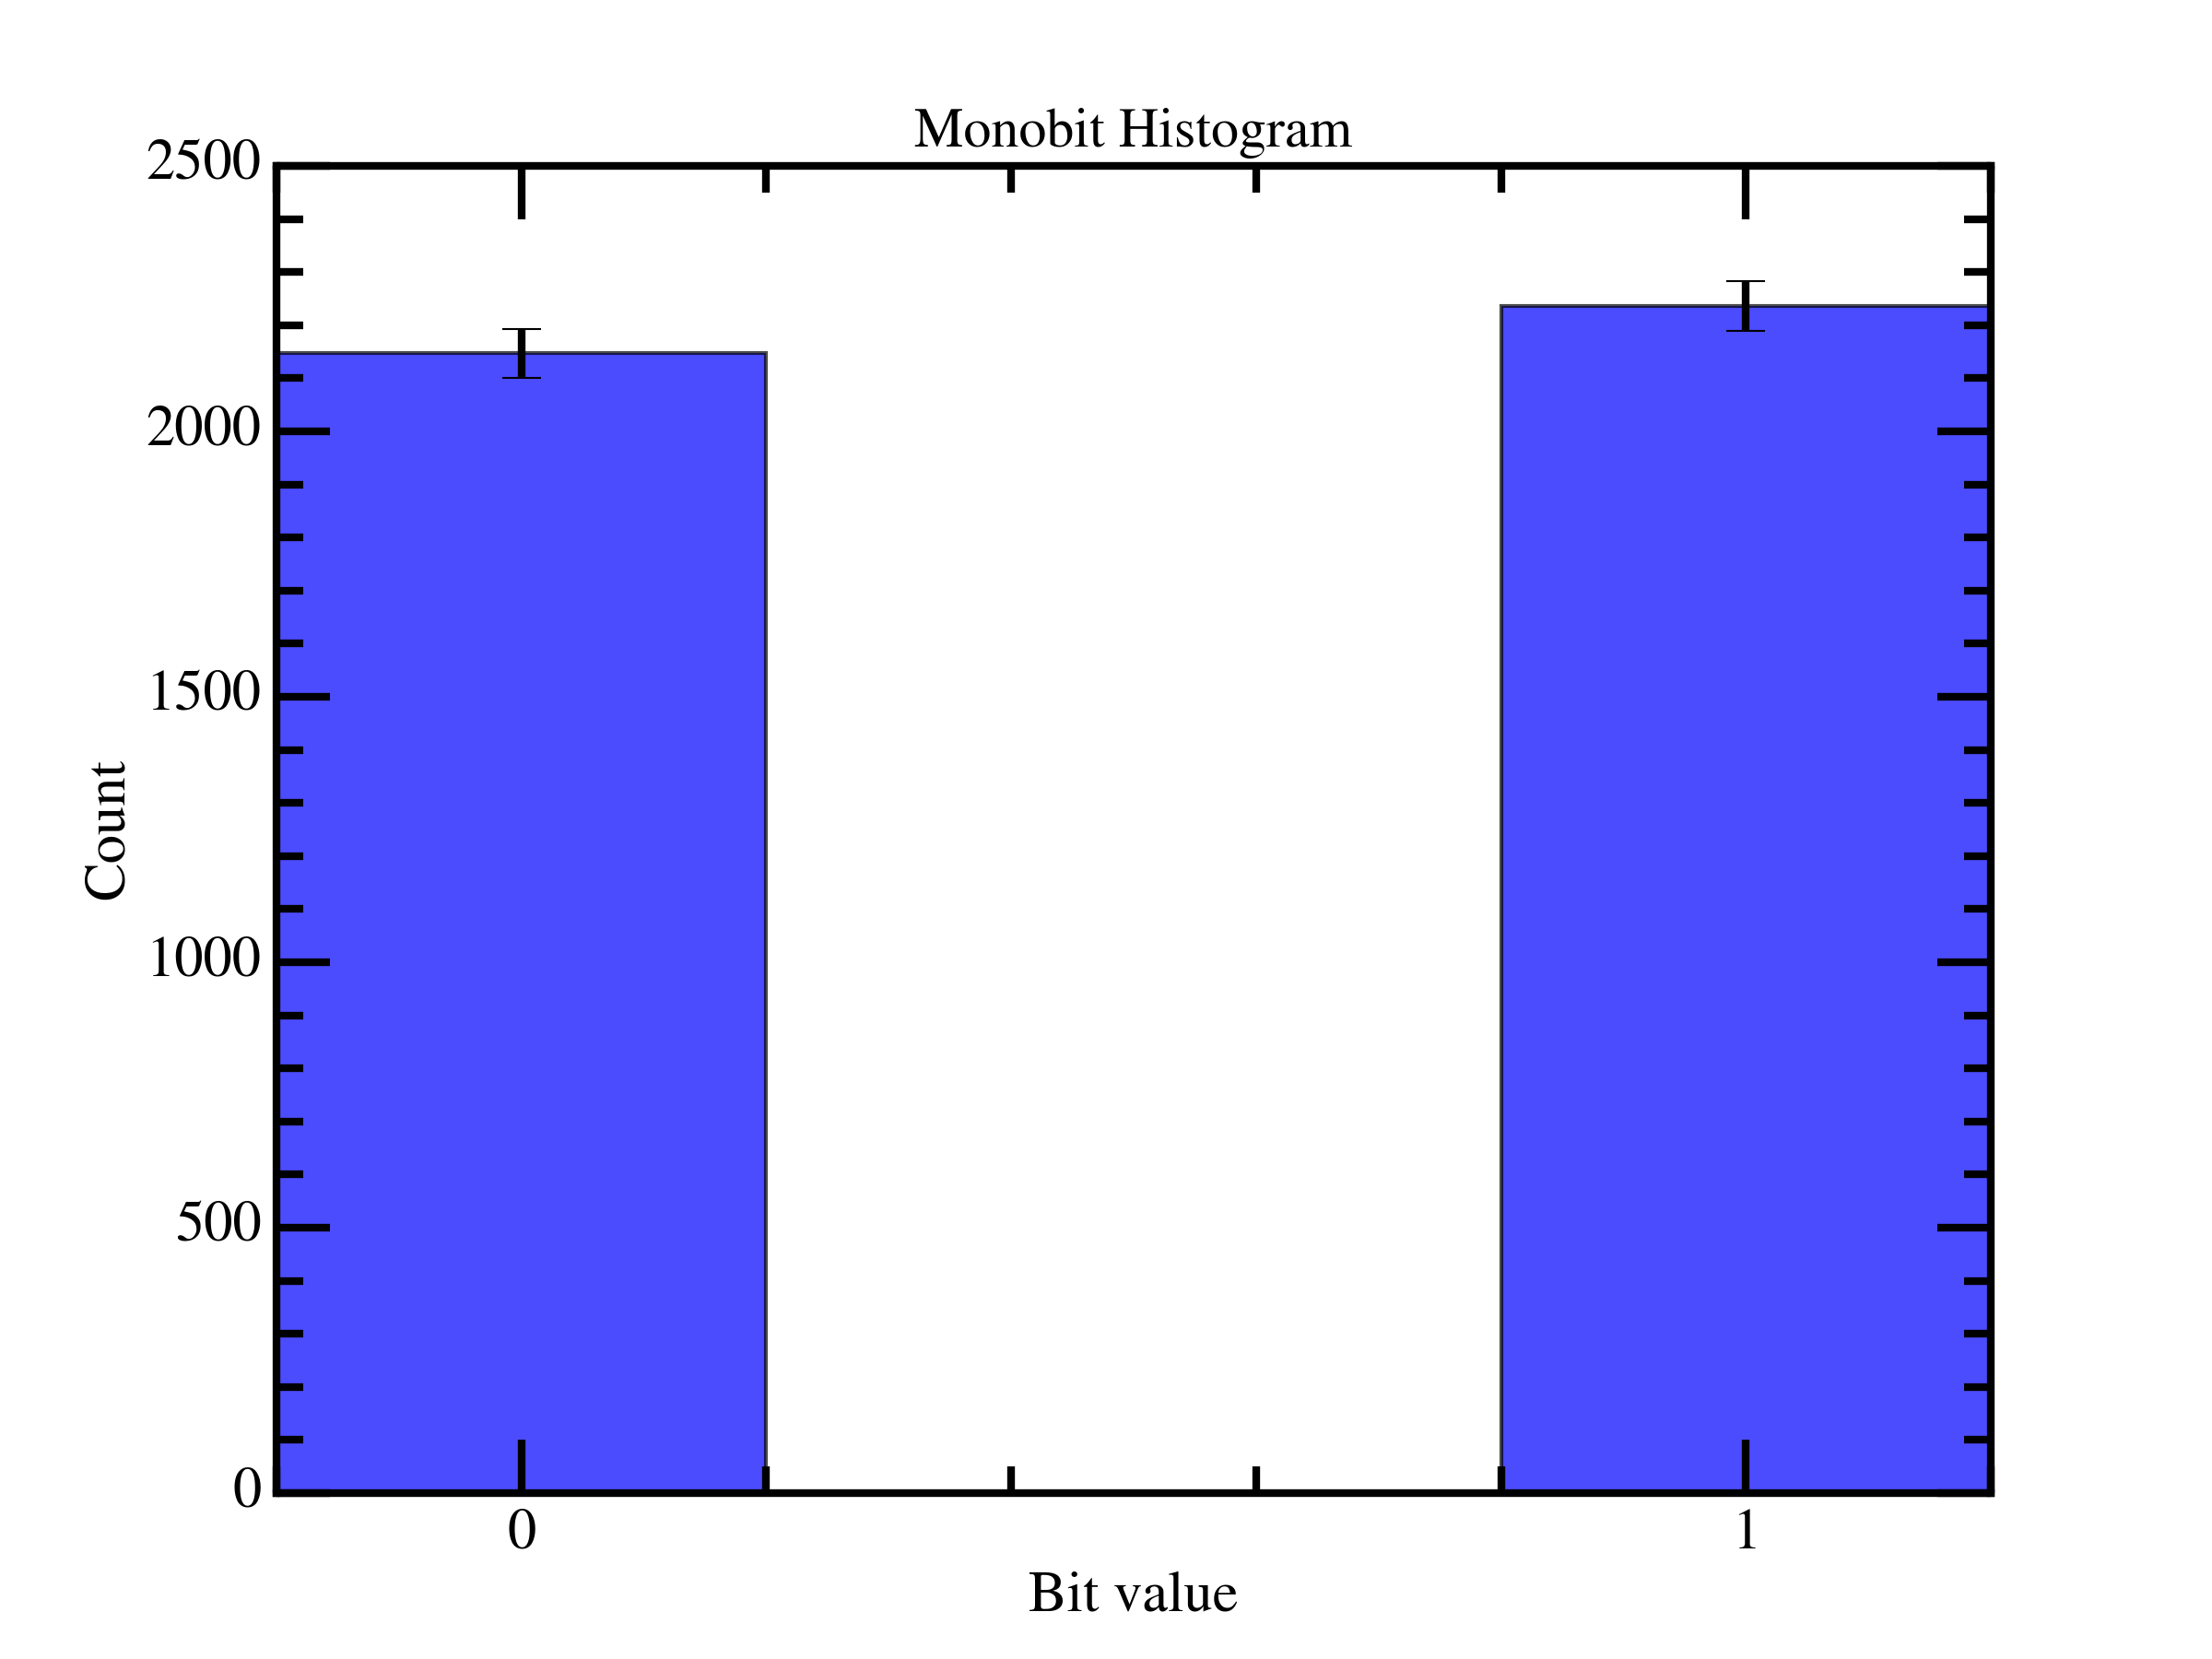
\includegraphics[width=0.45\textwidth]{figure/plot_monobit_histogram.png}
\caption{Histogram of the binary sequence. The plot shows that the count of 1 and 0 is roughly equal, indicating that the data is random.}
\label{fig:monobit_histogram}

\end{figure}

Next, we show the autocorrelation function of the binary sequence. The plot shows that the autocorrelation function decays to zero, indicating that the data is random.
\begin{figure}
\centering
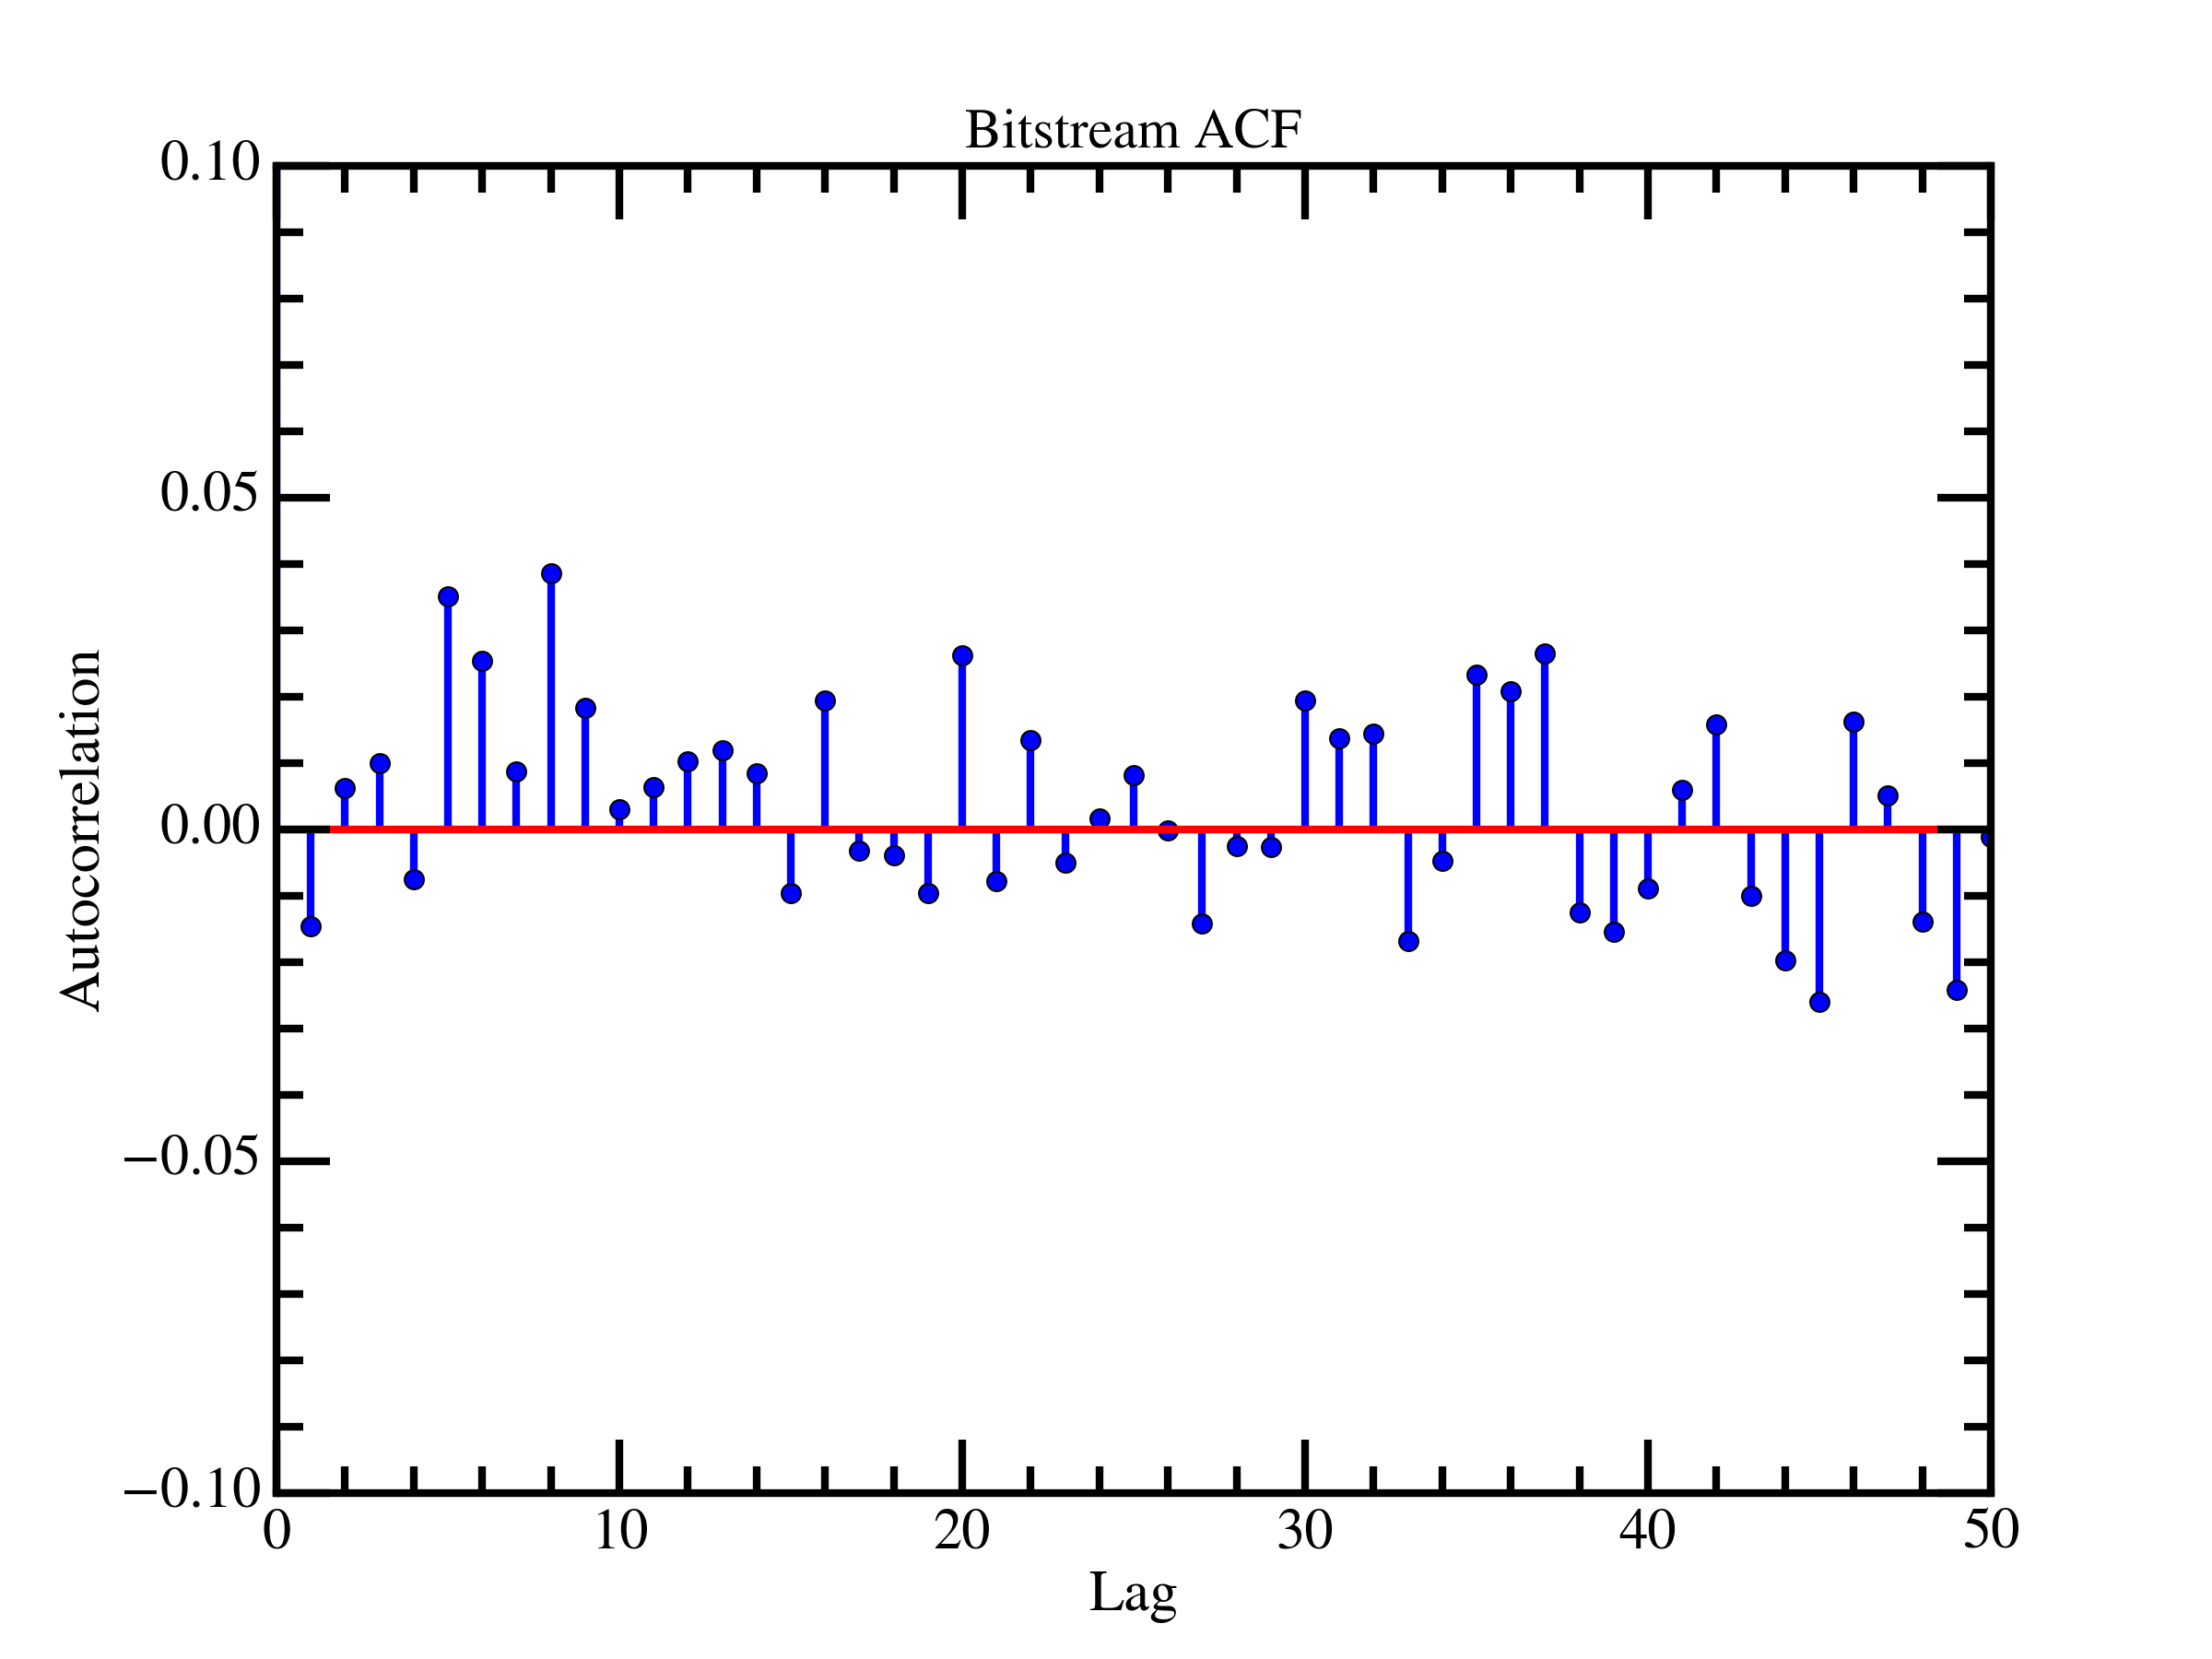
\includegraphics[width=0.45\textwidth]{figure/plot_autocorrelation.png}
\caption{Autocorrelation function of the binary sequence against the time lag. The plot shows that the autocorrelation function decays to zero, indicating that the data is random.}
\label{fig:autocorrelation}
\end{figure}

Next, we show the 4-bit and 6-bit binary sequence. The plot shows that the probability of each bit is roughly equal, indicating that the data is random.
\begin{figure}
\centering
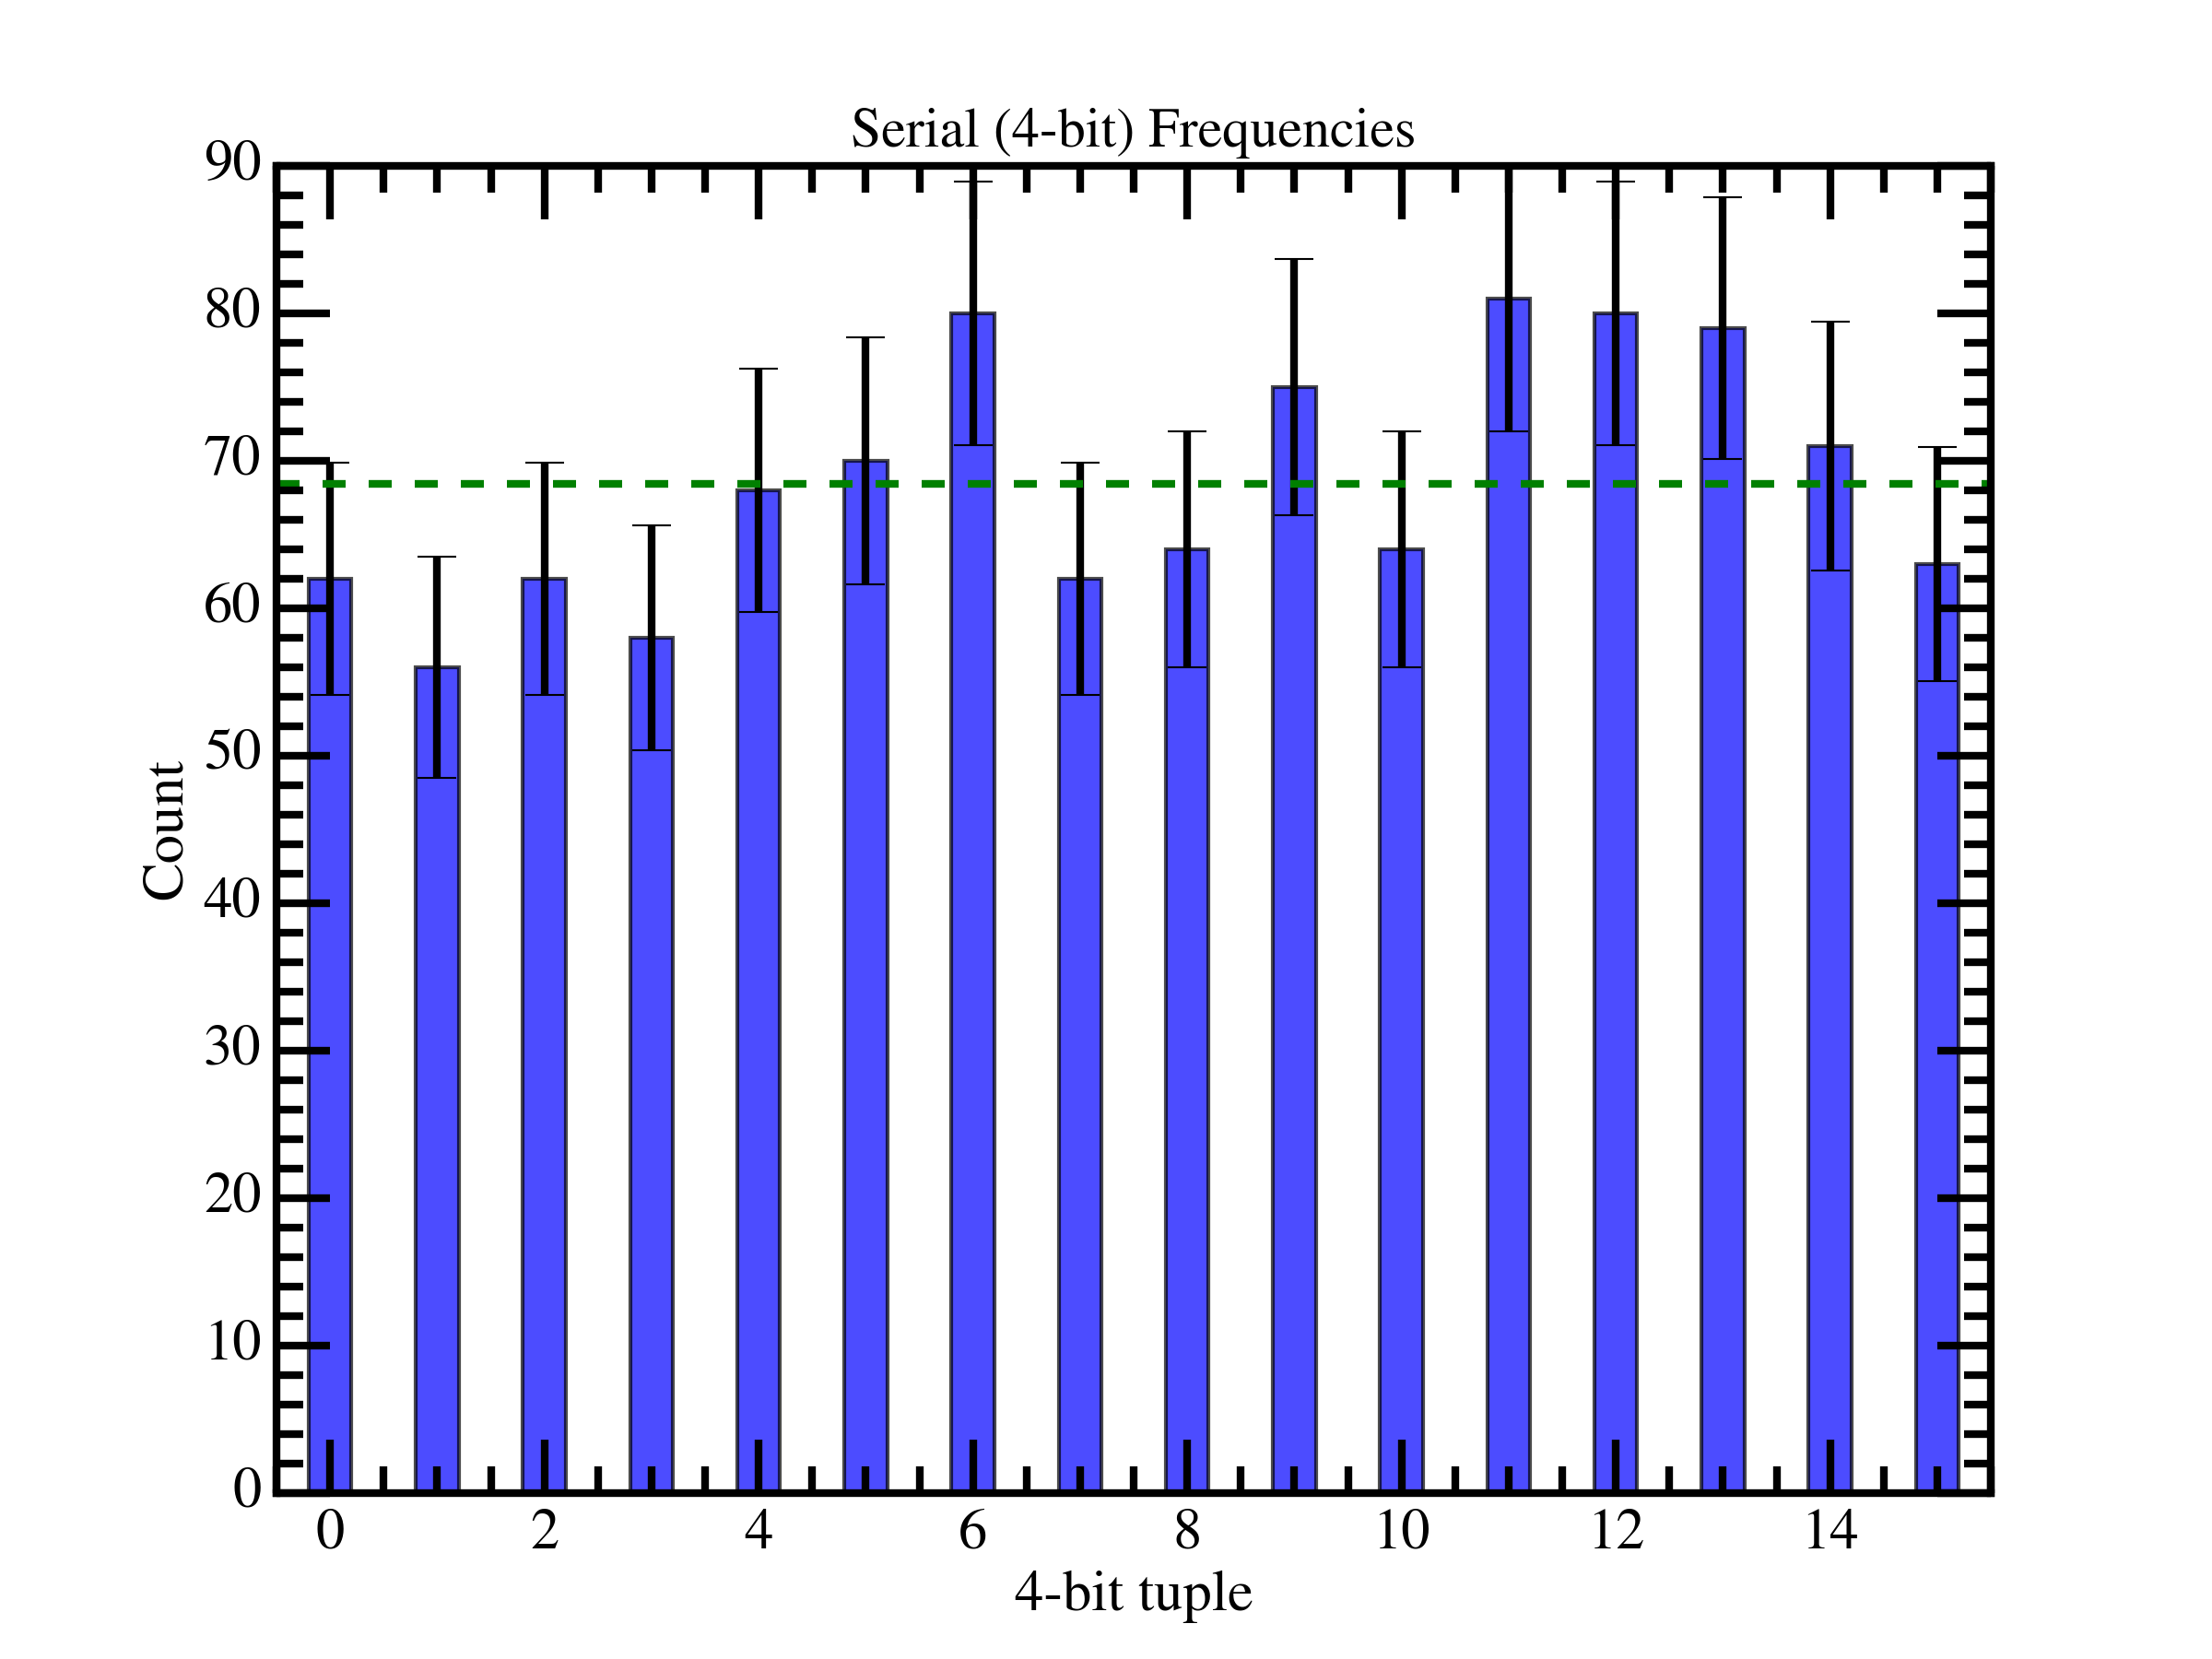
\includegraphics[width=0.45\textwidth]{figure/plot_serial_4bit_frequencies.png}
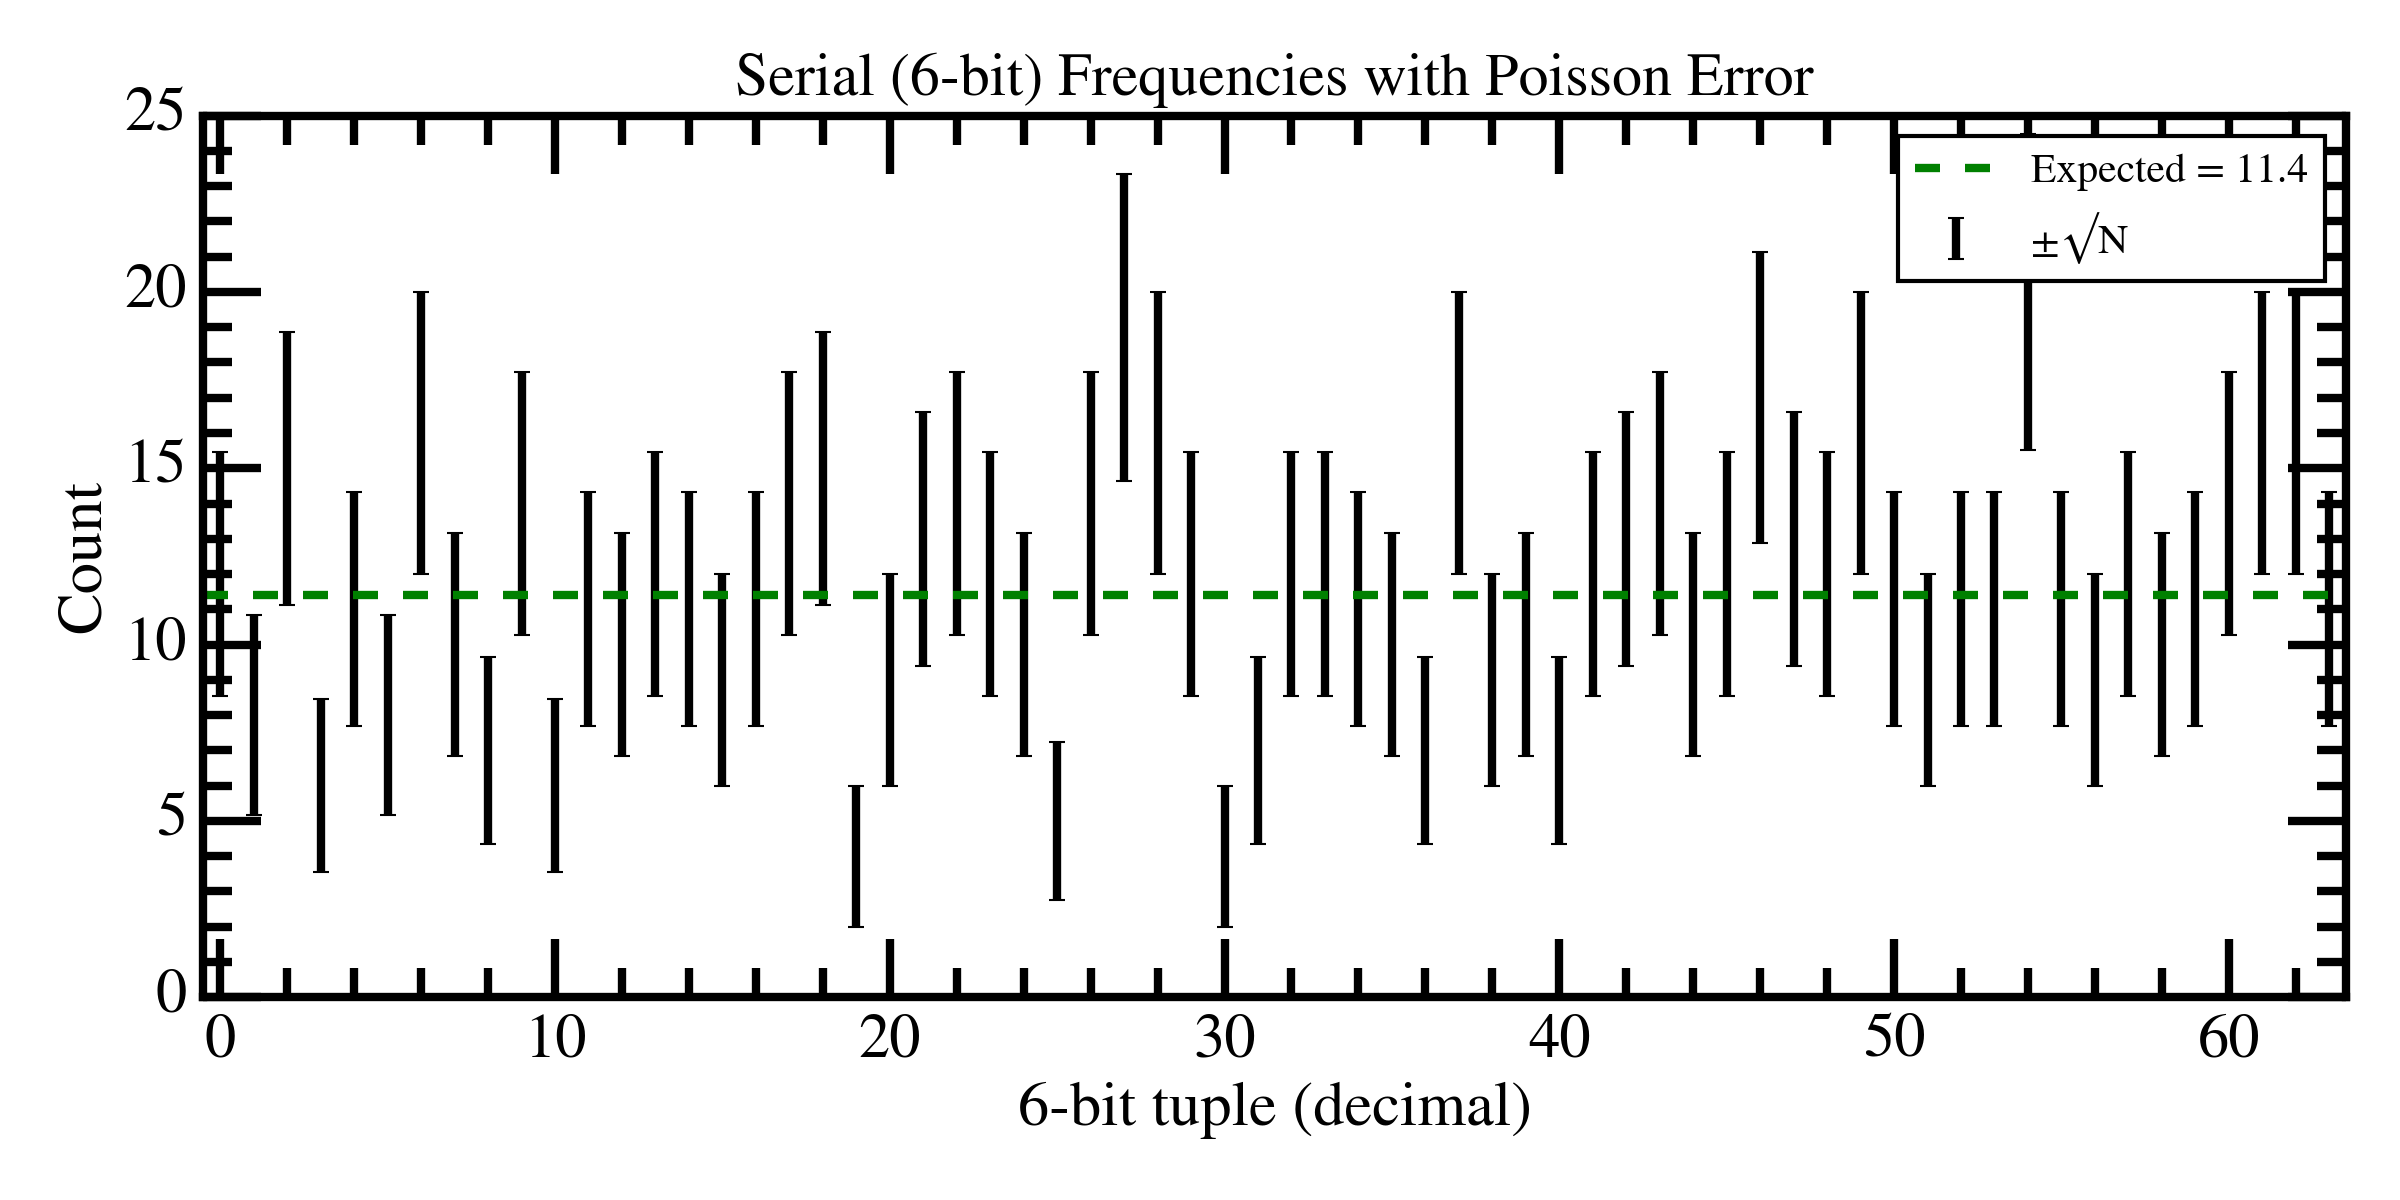
\includegraphics[width=0.45\textwidth]{figure/plot_serial_6bit_frequencies.png}
\caption{4-bit and 6-bit binary sequence. The plot shows that the probability of each bit is roughly equal, indicating that the data is random.}
\label{fig:serial_4bit_6bit}
\end{figure}

Next, we show the compression ratio of the binary sequence. With the compression algorithm, we have a compression ratio of $1.009$. The reason for the compression ratio being greater than 1 is that the compression algorithm adds header information to the compressed data. 

Next, we show the entropy of the binary sequence. 

Next, we show the result of the Lempel-Ziv complexity test. 

Lastly, we show the dependence of the probability of getting a 1 in the sequence on the angle of the detectors. The plot shows that the probability of getting a 1 in the sequence is roughly equal for all angles, indicating that the angle does not have a significant effect on the random nature of the data.
\begin{figure}
\centering
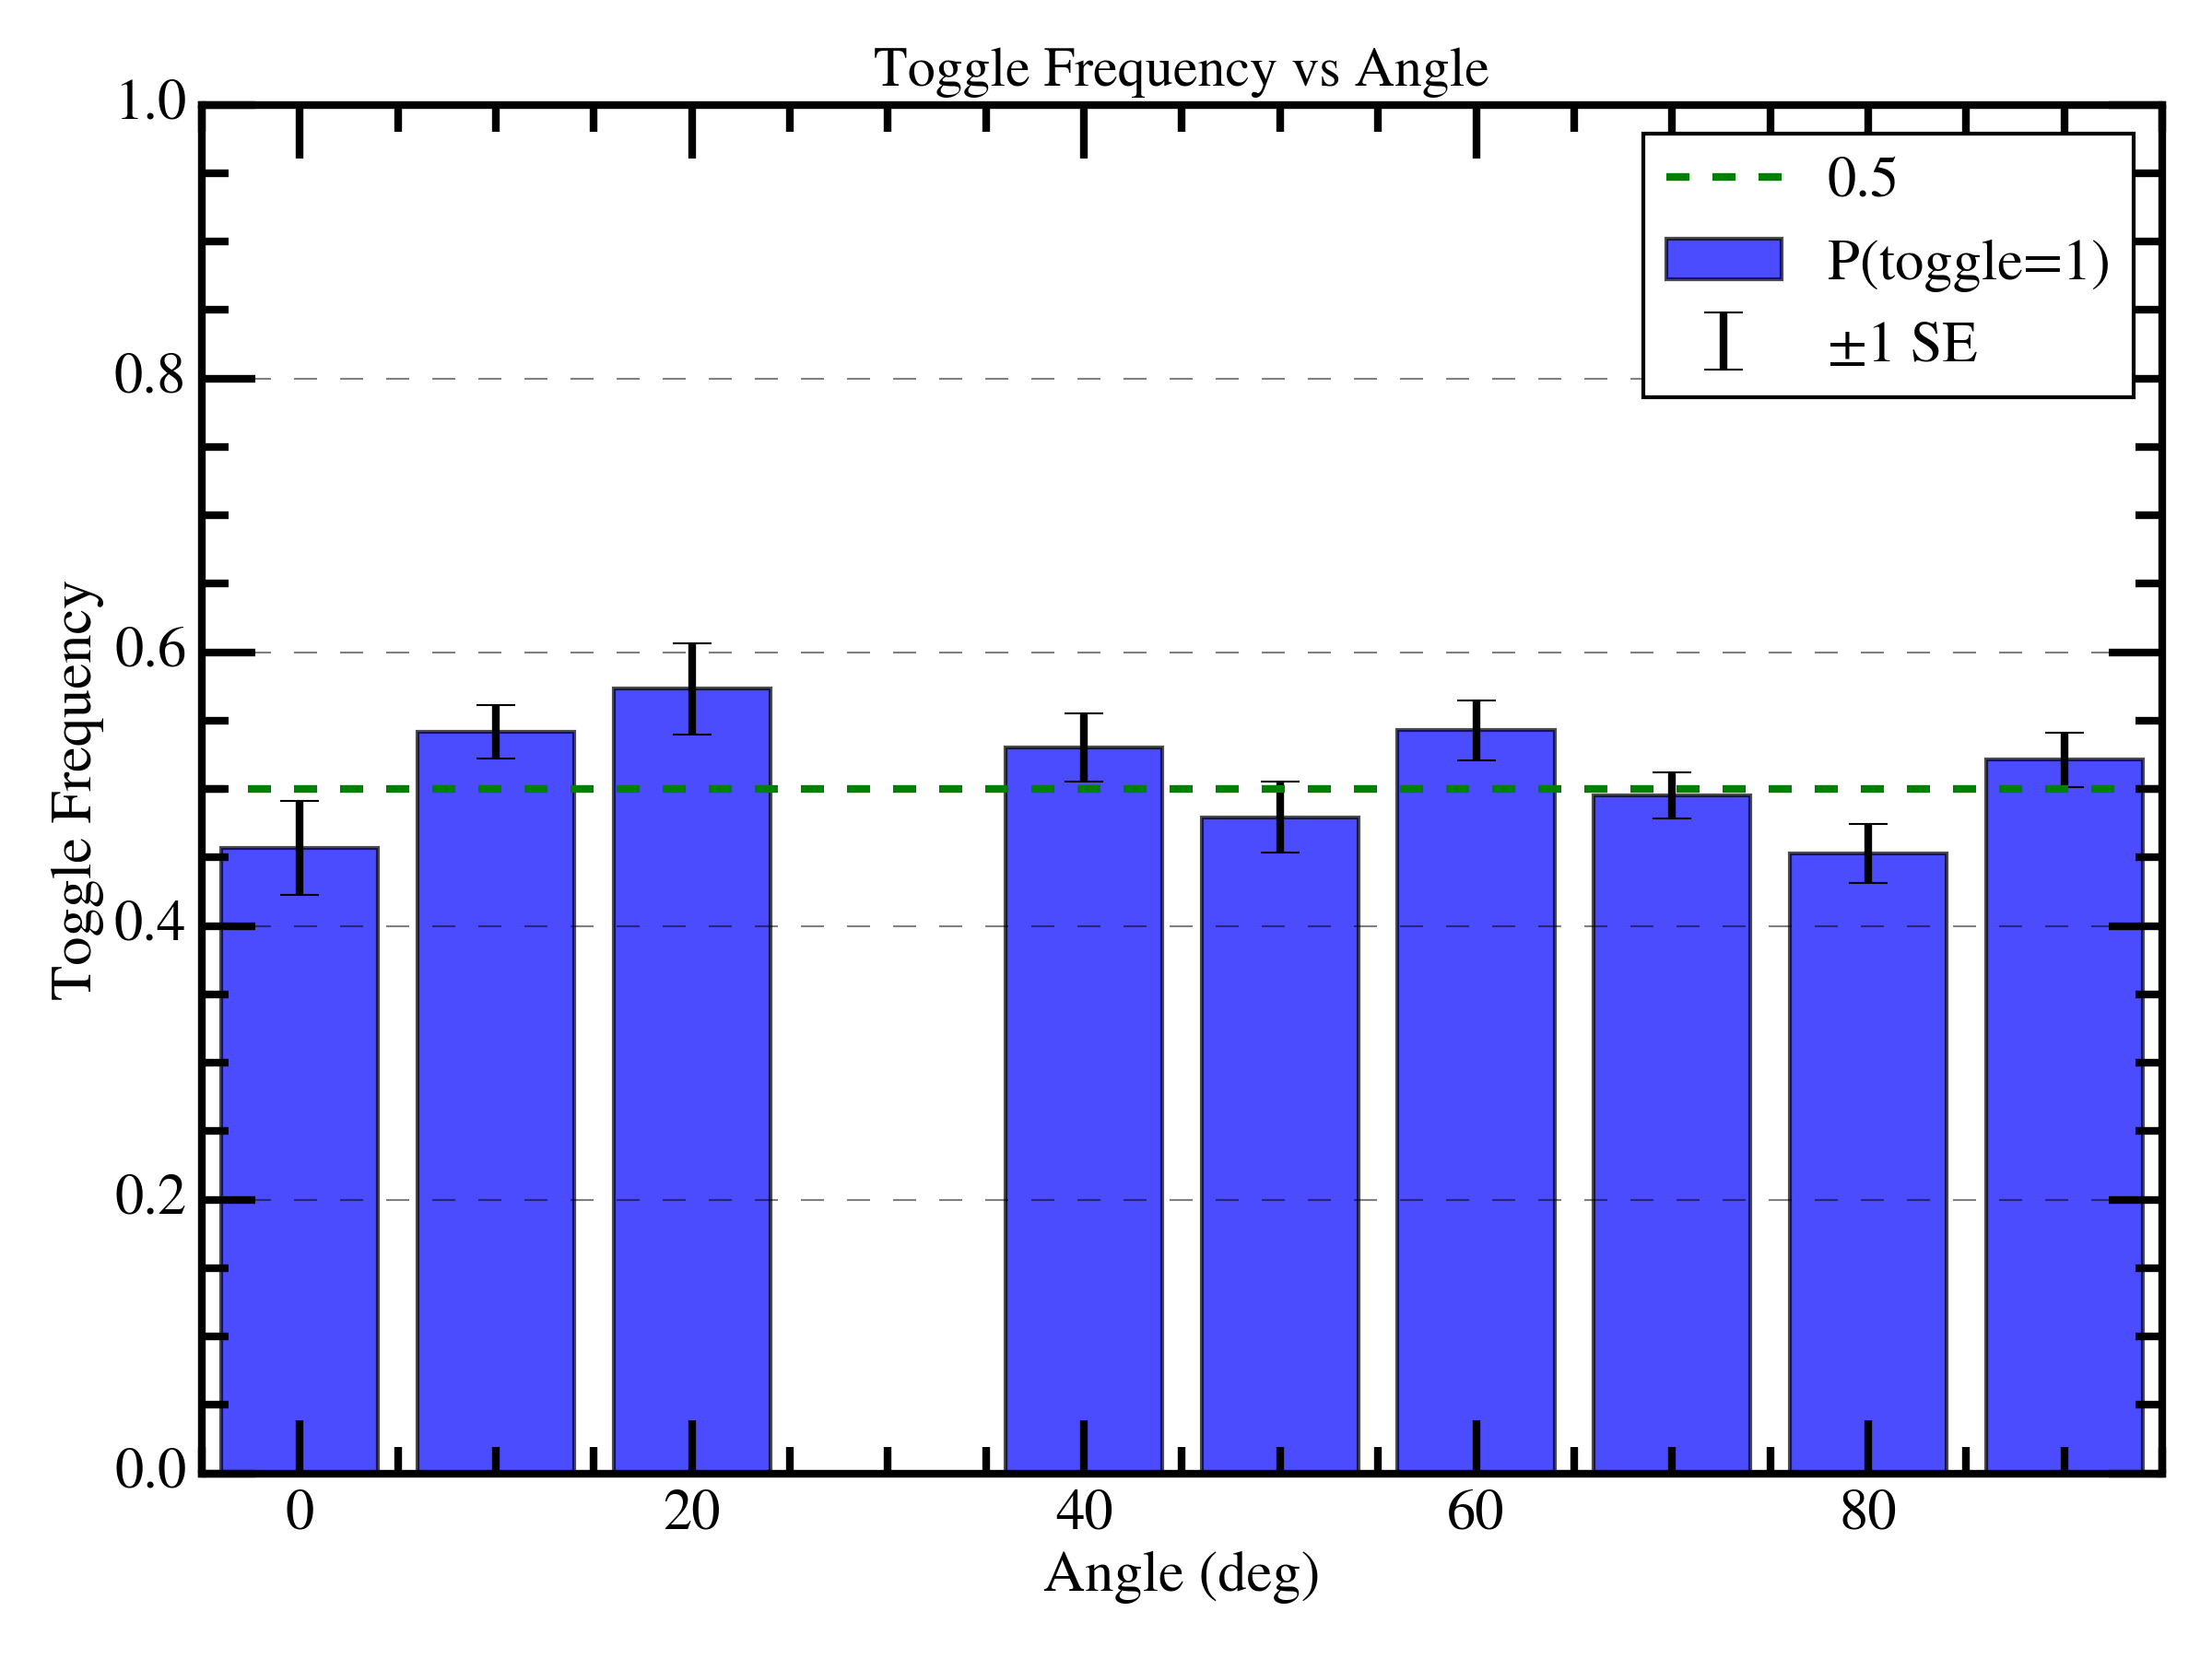
\includegraphics[width=0.45\textwidth]{figure/plot_toggle_frequency_by_angle.png}
\caption{Dependence of the probability of getting a 1 in the sequence on the angle of the detectors. The plot shows that the probability of getting a 1 in the sequence is roughly equal for all angles, indicating that the angle does not have a significant effect on the random nature of the data.}
\label{fig:angle_dependence}
\end{figure}

\section{Conclusion}
In conclusion, the analysis shows that the muon detection process is indeed random. The results of the statistical tests, including the autocorrelation function, sequence test, compression test, entropy test, chi-squared test, Lempel-Ziv complexity test, Kolmogorov-Smirnov test, and runs test, all indicate that the data is random. The analysis also shows that the angle of the detectors does not have a significant effect on the random nature of the data.

The results of the analysis are consistent with the expected behavior of a random process. The analysis also shows that the muon detection process is not affected by the angle of the detectors. The muon detection process is a random process, and the data collected by the Cosmic Muon Detector at MIT is indeed random.

The application of a true random number generator is important in many fields, including cryptography, simulations, and statistical analysis. The results of this analysis show that the muon detection process can be used as a source of true random numbers. 

\subsection{Uncertainty Analysis}
The uncertainty in the data is primarily due to the statistical nature of the muon detection process. The number of muon detection events is subject to statistical fluctuations, which can affect the results of the analysis. The uncertainty in the probability of getting a 1 in the sequence can be estimated using the binomial distribution. The uncertainty in the autocorrelation function can be estimated using the standard error of the mean. The uncertainty in the compression ratio can be estimated using the standard deviation of the compression ratio. The uncertainty in the entropy can be estimated using the standard deviation of the entropy. The uncertainty in the Lempel-Ziv complexity can be estimated using the standard deviation of the Lempel-Ziv complexity.


\vfill\null

\begin{acknowledgments} The author gratefully acknowledges their lab partner V. Tran for their invaluable assistance. The author also thanks the 8.13 teaching team for their guidance in the lab. This work was supported by the MIT Department of Physics. 
\end{acknowledgments}

\bibliographystyle{abbrv}
\bibliography{ref}
\end{document}

